% !TEX encoding = UTF-8 Unicode
\documentclass[italian,a4paper]{article}
\usepackage[tight,nice]{units} %unità di misura
\usepackage{babel,amsmath,amssymb,amsthm,graphicx,url,textcomp,gensymb, ctable}
\graphicspath{{./grafici/}}
\usepackage[text={5.5in,9in},centering]{geometry}
\usepackage[utf8x]{inputenc}
\usepackage[T1]{fontenc}
\usepackage{ae,aecompl}
\usepackage[small,bf]{caption}
\frenchspacing
\pagestyle{plain}
%------------- eliminare prime e ultime linee isolate
\clubpenalty=9999%
\widowpenalty=9999
%--- definizione numerazioni
\renewcommand{\theequation}{\thesection.\arabic{equation}}
\renewcommand{\thefigure}{\arabic{figure}}
\renewcommand{\thetable}{\arabic{table}}
\addto\captionsitalian{\renewcommand{\figurename}{Grafico}}
%------------- ridefinizione simbolo per elenchi puntati: en dash
\renewcommand{\labelenumi}{\textbf{\arabic{enumi}.}}
\renewcommand{\labelitemi}{\textbf{- }}
\setlength{\abovecaptionskip}{\baselineskip}   % 0.5cm as an example
\setlength{\floatsep}{2\baselineskip}
\setlength{\belowcaptionskip}{\baselineskip}   % 0.5cm as an example
%--------- comandi insiemi numeri complessi, naturali, reali e altre abbreviazioni
\renewcommand{\leq}{\leqslant}
\renewcommand{\geq}{\geqslant}
%--------- porzione dedicata ai float in una pagina:
\renewcommand{\textfraction}{0.05}
\renewcommand{\topfraction}{0.95}
\renewcommand{\bottomfraction}{0.95}
\renewcommand{\floatpagefraction}{0.35}
\setcounter{totalnumber}{5}
%-------------------------ambiente codice
\usepackage{listings}
\lstset{language=C++,inputencoding=utf8,breaklines=true,extendedchars=true, basicstyle=\small, columns=flexible, linewidth=\textwidth, lineskip=1pt, breakatwhitespace=true, lastline=99999, showstringspaces=false}
\lstloadlanguages{C++}
%-----------------------elenco compatto
\newenvironment{packed_item}{
\begin{itemize}
  \setlength{\itemsep}{1pt}
  \setlength{\parskip}{0pt}
  \setlength{\parsep}{0pt}
}{\end{itemize}}
\newenvironment{packed_enum}{
\begin{enumerate}
  \setlength{\itemsep}{1pt}
  \setlength{\parskip}{0pt}
  \setlength{\parsep}{0pt}
}{\end{enumerate}}

%------------shortcuts
\renewcommand{\a}{\alpha}
\renewcommand{\l}{\lambda}
\newcommand{\s}{\sigma}
\renewcommand{\d}{\delta}
\newcommand{\D}{\Delta}
\renewcommand{\r}{\rho}
\newcommand{\Am}{$^{241}$Am}
\newcommand{\Cm}{$^{244}$Cm}
\newcommand{\Pu}{$^{239}$Pu}

%---------
%
%---------
\begin{document}
\title{Interazione di particelle cariche con la materia}
\author{\normalsize Ilaria Brivio (582116)\\%
\normalsize \url{brivio.ilaria@tiscali.it}%
\and %
\normalsize Matteo Abis (584206)\\ %
\normalsize \url{webmaster@latinblog.org}
\date{\today}
\and
\normalsize Lorenzo Rossato(579393)\\ %
\normalsize \url{supergiovane05@hotmail.com}}
\date{\today}
\maketitle
%------------------
\section{Obiettivo dell'esperimento}
Verificare che per particelle $\a$ che si propagano in uno stesso mezzo la posizione del picco di Bragg \`e indipendente dalla loro energia.

Verificare la validit\`a della legge di Bragg-Kleman
\begin{equation*}
\frac{R_1}{R_2} = \frac{\r_2 \sqrt{A_1}}{\rho_1 \sqrt{A_2}}
\end{equation*}
confrontando il range di particelle $\a$ in mezzi di densit\`a $\r$ diversa.
\section{Apparato strumentale}
Abbiamo utilizzato il banco di laboratorio C3.
\subsection*{Descrizione dell'apparato}
L'apparato sperimentale \`e costituito da una camera di ionizzazione contenente una miscela di Ar e CO$_2$ (0.5\%), al cui interno \`e presente una sorgente di particelle $\a$ composta da \Am, \Cm, \Pu. Riportiamo nella tabella seguente i parametri di decadimento\footnote{
Fonti:\\
\begin{tabular}[h!]{cl}
\Am&	M.S. Basunia, \textit{Nuclear Data Sheets}, 107, 3323 (2006)\\
\Cm&	Balraj Singh, \textit{Nuclear Data Sheets}, 109, 2439 (2008)\\
\Pu&	E. Browne, \textit{Nuclear Data Sheets}, 98, 665 (2003)
\end{tabular}
} di tali isotopi:
\vskip -.2cm
\begin{table}[h!]\centering
\renewcommand{\arraystretch}{1.1}
\begin{tabular}{*3{lc}}
\multicolumn{2}{c}{\Am}&		\multicolumn{2}{c}{\Cm}&		\multicolumn{2}{c}{\Pu}\\\midrule[.15em]
$E_\a$ (MeV) &		\%&		$E_\a$ (MeV)&	\%&		$E_\a$ (MeV)&		\%\\
5.48556(12)&		84.8&		5.80477(5)&	76.90&		5.15659(14)&		70.77\\
5.44280(13)&		13.1&		5.76264(3)&	23.10&		5.1443(8)&		17.11\\
5.388&			1.660&		&		&		5.1055(8)&		11.94\\\hline
\multicolumn{2}{l}{media pesata (MeV)}& & & & \\
5.47831&	&			5.79504&	&		5.14837& \\\hline
\multicolumn{2}{l}{vita media $\tau$ (y)}& & & & \\
432&		&			18.1&		&		24110&	
\end{tabular}
\caption{Parametri di decadimento $\a$ per i tre isotopi contenuti nella sorgente.}
\label{isotopi}
\end{table}
\newpage
I dati raccolti nella nostra esperienza saranno riferiti sostanzialmente ai tre decadimenti di energia pi\`u probabile. Nella procedura di calibrazione in energia e stima della risoluzione della camera abbiamo per\`o scelto di considerare le medie delle energie di ciascun ramo di decadimento, pesate secondo le percentuali indicate sopra.

Il rivelatore presente nella camera \`e connesso, nell'ordine, a un amplificatore lineare, un convertitore FADC, e quindi a un computer dal quale \`e possibile raccogliere i dati e impostare la pressione del gas, agendo su un'apposita valvola a spillo.

Per la parte di messa a punto dell'elettronica ci siamo serviti inoltre di un oscilloscopio manuale.
\subsection*{Messa a punto dell'apparato}
Per prima cosa abbiamo impostato lo shaping-time dell'amplificatore a \unit[0.5]{\micro s}. Abbiamo quindi selezionato guadagni coarse e fine rispettivamente di 100 e 1.40 e connesso l'oscilloscopio all'uscita unipolare dell'amplicatore per poter monitorare il segnale trasmesso. In questo modo abbiamo verificato che l'ampiezza massima dei segnali registrati alla pressione di \unit[600]{mbar} restasse sotto i \unit[2.5]{V} e che il segnale tornasse a zero in modo corretto.

In una seconda fase abbiamo cercato di individuare la soglia di potenziale che permettesse di ridurre al 25-30~\% del totale gli eventi di fondo, dovuti a eventi di riflessione delle particelle o a scariche elettriche all'interno della camera. Fissata la pressione a \unit[600]{mbar}, abbiamo registrato 50 eventi per ciascun valore di soglia minima del convertitore FACD e abbiamo contato quanti di questi fossero spuri:
\begin{table}[h!]\centering
\begin{tabular}{*2c}
soglia (V)&  eventi spuri\\\hline
1.20&		6 (12 \%)\\
1.12&		10 (20 \%)\\
0.96&		10 (20 \%)\\
0.80&		15 (30 \%)\\
0.76&		14 (28 \%)
\end{tabular}
\caption{Misure di prova del numero di eventi spuri registrati a \unit[600]{mbar} variando la soglia di conversione del FADC.}
\end{table}\\
Dalle misure effettuate abbiamo ritenuto opportuna una soglia di \unit[0.76]{V}.

Con lo stesso metodo abbiamo realizzato 50 misure di prova variando la pressione di camera fino a \unit[400]{mbar}, scegliendo di volta in volta la soglia pi\`u opportuna. Riportiamo di seguito i valori trovati, assieme ad una stima per eccesso del canale $c_N$ a partire dal quale l'acquisizione registra solo segnale di fondo. Per completezza indichiamo inoltre il numero di eventi spuri registrati durante la presa dati.
\begin{table}[h!]\centering
\begin{tabular}{*5c}
$P$ (mbar)&	soglia (V)&	inizio fondo& 	eventi spuri / 50&	eventi spuri / 1500\\
&		&		&		(prova)&		(presa dati)\\\hline
600&		0.76&		65&		14 (28 \%)&		485 (32.3 \%)\\
550&		0.76&		70&		14 (28 \%)&		474 (31.6 \%)\\
500&		0.64&		75&		15 (30 \%)&		502 (33.5 \%)\\
450&		0.64&		75&		17 (34 \%)&		508 (33.9 \%)\\
400&		0.64&		80&		15 (30 \%)&		516 (34.4 \%)
\end{tabular}
\caption{Risultati delle misure di prova effettuate a diverse pressioni. Il valore della soglia di conversione riportato \`e quello assunto come definitivo.}
\end{table} 
\subsection*{Condizioni di presa dati}
Abbiamo fatto variare la pressione del gas nella camera da 400 a \unit[600]{mbar} a passi di 50, e per ciascun valore abbiamo raccolto una serie di 1500 eventi, controllando che la percentuale di eventi di fondo restasse sempre attorno al 25-30~\%.
Riassumiamo di seguito i parametri impostati nella presa dati:
\begin{table}[h!]\centering
\begin{tabular}{rll}
amplificatore&		shaping time&		\unit[0.5]{\micro s}\\
&			guadagno coarse&	$\times 100$\\
&			guadagno fine&		$\times 1.40$\\
&			polarit\`a&		positiva\\
FADC&			soglia min.&		\unit[0.76]{V} per 600, \unit[550]{mbar}\\
&			&			\unit[0.64]{V} per 500, 450, \unit[400]{mbar}\\
&			nr. canali&		128\\
acquisizione&		N eventi&		1500
\end{tabular}
\end{table}
\section{Analisi dati e risultati ottenuti}
Da ciascun evento abbiamo estratto le seguenti informazioni:
\begin{packed_enum}
\item altezza del fondo $\bar{f}$, calcolato come media sui canali non interessati dal picco del segnale:
\begin{equation*}
\bar{f} = \frac{1}{128 - N - 1} \sum_{i=N}^{128}{c_i}
\end{equation*}
dove $c_i$ \`e il contenuto dell'$i$-esimo canale e $c_N$ il bin da cui si ha solo fondo.

\item altezza $h_{\max}$ e posizione $t_{\max}$ del picco di Bragg. Dalla prima abbiamo sottratto $\bar{f}$.

\item l'integrale della curva privata del fondo, proporzionale all'energia $E_\a$ della particella $\a$ che ha prodotto il segnale.

\item durata $\D t$ dell'evento, che abbiamo assunto pari alla larghezza della curva al 45~\% della sua altezza.

\item frazione di energia residua $E_{\text{res}}$ oltre il massimo di Bragg. Questo valore servir\`a per verificare che la velocit\`a delle particelle $\a$ nella camera sia molto minore di quella degli elettroni.
\end{packed_enum}

\subsection{Calibrazione in energia e risoluzione dell'apparato}
Per ciascun valore della pressione abbiamo realizzato un istogramma dei valori degli integrali, da cui \`e possibile distinguere tre decadimenti con energie distinte, corrispondenti ai tre isotopi della sorgente.
Per ottimizzare la definizione dei picchi senza tuttavia alterarne la forma, abbiamo scelto di suddividere l'intervallo di valori considerato (5000 - 7000) in 150 canali.
Riportiamo a titolo di esempio il grafico per la pressione di \unit[550]{mbar}.
\begin{figure}[h!]\centering
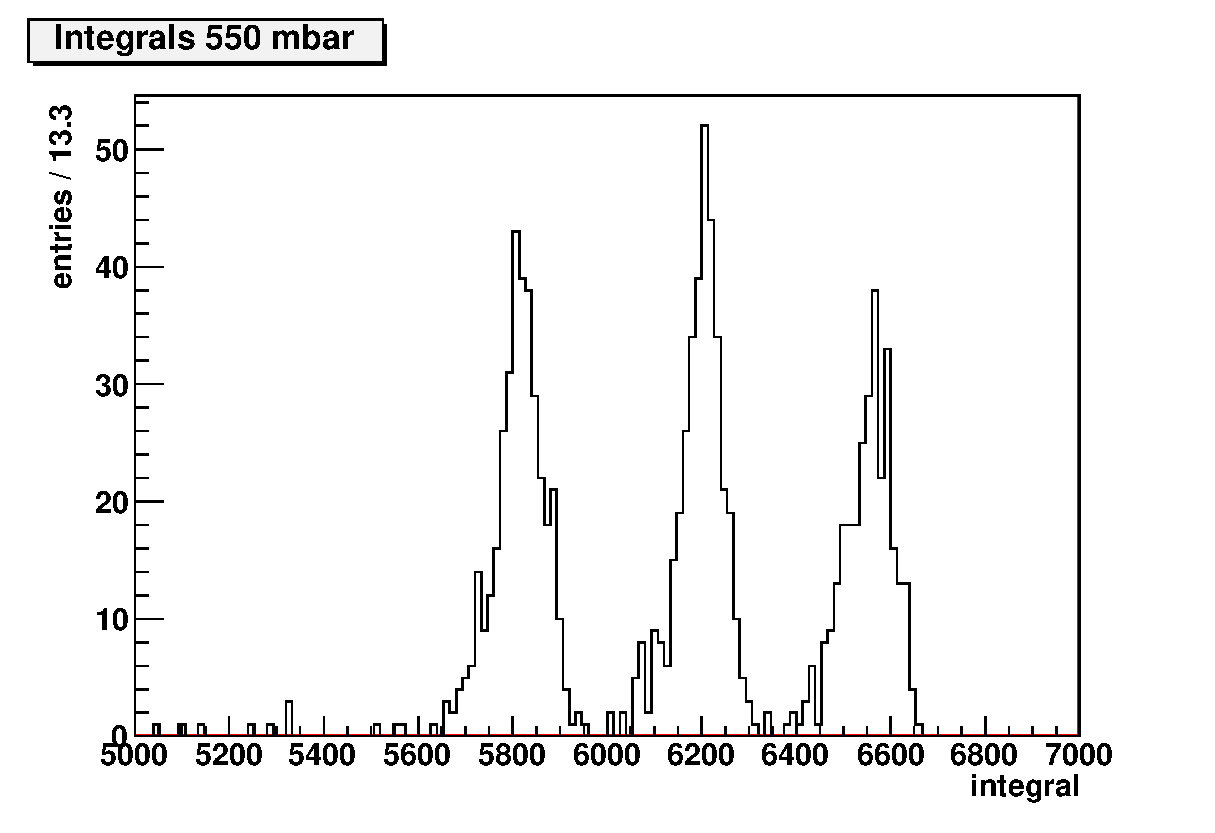
\includegraphics[width=0.8\textwidth]{550_integral.eps}
\caption{Istogramma degli integrali per gli eventi registrati con pressione di \unit[550]{mbar}. I tre picchi visibili corrispondono all'energia del decadimento pi\`u probabile, rispettivamente per \Pu, \Am, \Cm.}
\label{int_hist}
\end{figure}\\
A \unit[400]{mbar} le particelle emesse dal curio non vengono fermate nella camera e di conseguenza il loro picco non risulta visibile nell'istogramma degli integrali. Per questo motivo non impiegheremo i dati raccolti a questa pressione nella procedura descritta oltre.

Per la calibrazione in energia della camera abbiamo calcolato il valore medio degli integrali di ciascuno dei tre gruppi di eventi e abbiamo posto i risultati in grafico, rapportandoli ai valori noti delle energie $E$.
Dato che ciascun isotopo della sorgente segue pi\`u di un ramo di decadimento, \`e realistico supporre che i picchi visibili nell'istogramma siano piuttosto convoluzioni dei due o tre picchi relativi alle energie di emissione pi\`u probabili. Per questo motivo abbiamo scelto di assumere come valore di $E$ la loro media, pesata secondo le percentuali riportate in tabella~\ref{isotopi}. 

% Il grafico seguente \`e quello relativo alla pressione di \unit[550]{mbar}.
\begin{figure}[h!]\centering
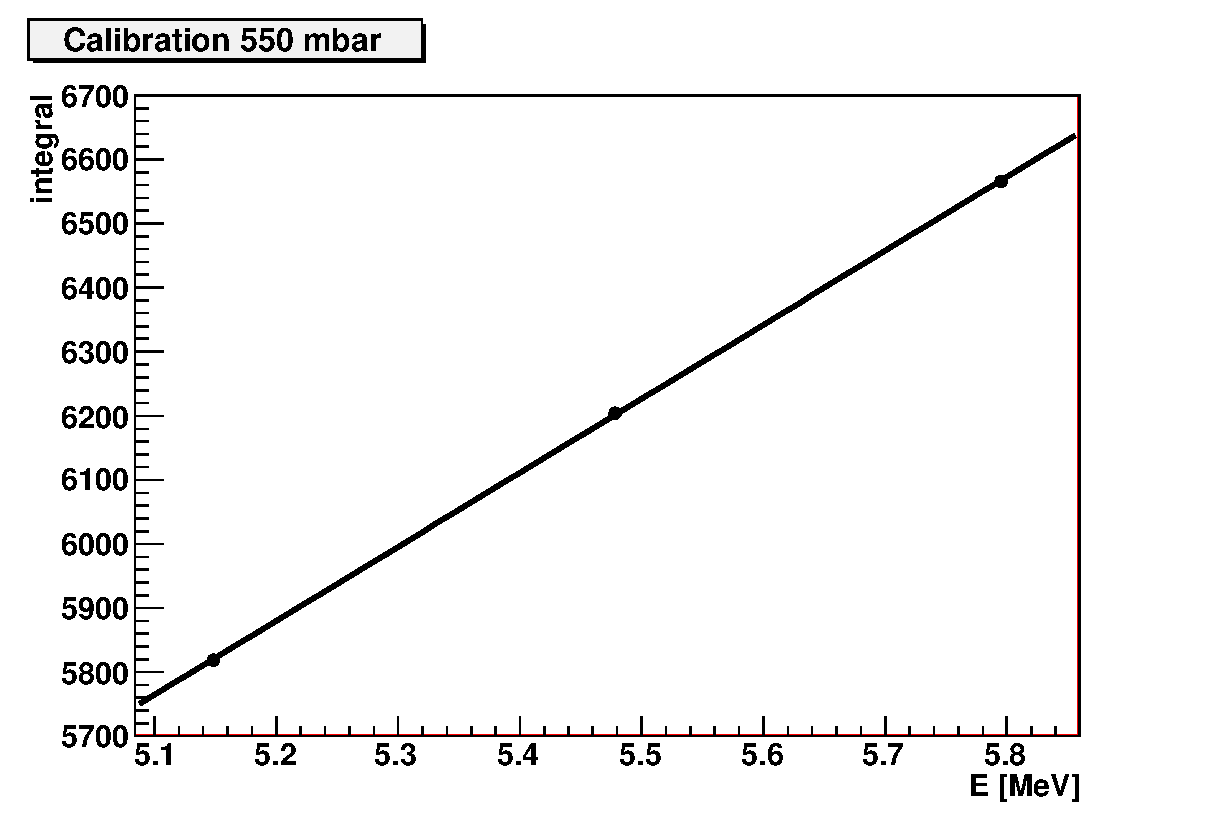
\includegraphics[width=0.8\textwidth]{550_calib.eps}
\caption{Grafico con valori dell'energia in ascissa (MeV) e integrali medi in ordinata per gli eventi registrati alla pressione di \unit[550]{mbar}. Le barre di errore non sono visibili perch\'{e} contenute entro le dimensioni del punto.}
\label{calib}
\end{figure}
\clearpage
Dal fit lineare dei grafici per ciascuna delle quattro pressioni abbiamo i seguenti parametri di proporzionalit\`a:
\begin{table}[h!]\centering
\begin{tabular}{*4c}
$P$ (mbar)&		pendenza (MeV$^{-1}$)&	intercetta&   	$\chi^2$\\\hline
450&			1055 $\pm$ 7&		358 $\pm$ 41&	3.87\\
500&			1097 $\pm$ 7&		147 $\pm$ 35&	2.81\\
550&			1155 $\pm$ 6&		-125 $\pm$ 32&	1.68\\
600&			1116 $\pm$ 5&		120 $\pm$ 27&	62.60	
\end{tabular}
\caption{Risultati della regressione lineare dei grafici con energie in ascissa e integrali medi in ordinata.}
\end{table}\\
% Il $\chi^2$ molto elevato per i dati a \unit[600]{mbar} \`e probabilmente dovuto alla marcata assimmetria dei picchi nell'istogramma. 
Per la stima della risoluzione abbiamo considerato la larghezza a mezza altezza di ciascun picco, estraendone il valore di $\D E / E$ dai parametri di calibrazione:
\begin{table}[h!]\centering
\renewcommand{\arraystretch}{1.1}
\begin{tabular}{*7c}
$P$ (mbar)& &	$E$ (keV)&	integrale&	larghezza &	$\D E$ (keV)& $\D E / E$\\\midrule[.15em]
450&	Pu&	5148&	    	5788 $\pm$ 4& 	147&		140&	0.03\\
&	Am&	5478&		6146 $\pm$ 4& 	133&		126&	0.02\\
&	Cm&	5795&		6472 $\pm$ 3&	120&		114&	0.02\\\hline
% & & & & & \\
500&	Pu&	5148&	    	5792 $\pm$ 3&  	133& 		122& 	0.02\\
&	Am&	5478&		6160 $\pm$ 3&  	133& 		122& 	0.02\\
&	Cm&	5795&		6501 $\pm$ 3&  	93& 		85& 	0.01\\\hline
% & & & & & \\
550&	Pu&	5148&	    	5819 $\pm$ 3&  	93& 		81& 	0.02\\
&	Am&	5478&		6204 $\pm$ 3&  	67& 		58& 	0.01\\
&	Cm&	5795&		6566 $\pm$ 2&  	67& 		58& 	0.01\\\hline
% & & & & & \\
600&	Pu&	5148&	    	5864 $\pm$ 2&  	107& 		96& 	0.02\\
&	Am&	5478&		6260 $\pm$ 3&  	80& 		72& 	0.01\\
&	Cm&	5795&		6586 $\pm$ 2&  	80& 		72& 	0.01
\end{tabular}
\caption{Risultati della procedura di calibrazione in energia e risoluzione della camera.}
\end{table}\\
\subsection{Indipendenza del picco di Bragg dall'energia}
Per ogni valore della pressione abbiamo suddiviso gli eventi in base alla loro energia e per ciascun gruppo abbiamo stimato l'altezza media del picco di Bragg ottenendo i risultati riportati di seguito.
% Gli errori sono calcolati analogamente a quelli sugli integrali.
\begin{table}[h!]\centering
\begin{tabular}{*4c}
$P$ (mbar)&		\Pu&			\Am&			\Cm\\\hline
400&			155.78 $\pm$ 0.12&    	154.80 $\pm$ 0.15&		\\
450&			167.46 $\pm$ 0.12&    	167.36 $\pm$ 0.14&    167.86 $\pm$ 0.13\\
500&			180.91 $\pm$ 0.16&    	180.92 $\pm$ 0.13&    180.85 $\pm$ 0.13\\
550&			193.47 $\pm$ 0.13&    	193.89 $\pm$ 0.11&    194.04 $\pm$ 0.14\\
600&			205.32 $\pm$ 0.15&    	206.17 $\pm$ 0.18&    206.86 $\pm$ 0.20
\end{tabular}
\caption{Valori medi dell'altezza del picco di Bragg.}
\end{table}
\newpage
Per verificare l'effettiva indipendenza del picco abbiamo calcolato le compatibilit\`a di ciascuna delle tre coppie di valori per ogni pressione:
\begin{table}[h!]\centering
\begin{tabular}{*4c}
$P$ (mbar)&	Am-Pu&	Am-Cm&		Cm-Pu\\\hline
400&		5.10&	&		\\
450&		2.26&	0.54&		2.62\\
500&		0.29&	0.05&		0.38\\
550&		2.98&	2.47&		0.84\\
600&		6.16&	3.63&		2.56
\end{tabular}
\caption{Compatibilit\`a tra le altezze del picco di Bragg per ciascuna coppia di sorgenti.}
\end{table}\\
Avendo ottenuto dei buoni valori di compatibilit\`a, possiamo ritenere verificata l'indipendenza dell'altezza del picco dall'energia della particella incidente. La presenza di compatibilit\`a superiori a 3 -- 4 nei dati acquisiti a 400 e \unit[600]{mbar} pu\`o essere dovuta a una sottostima degli errori.
\subsection{Stima della velocit\`a di drift degli elettroni}
Alla pressione di \unit[400]{mbar} le particelle $\a$ pi\`u energetiche, ossia quelle emesse dal \Cm, va a urtare l'anodo. Questi eventi possono essere facilmente identificati in un grafico del massimo di Bragg in rapporto all'integrale della curva. Nel nostro caso, come si pu\`o vedere dal grafico seguente, si trovano nella zona con integrale superiore a 5000 e picco inferiore a 149.
\begin{figure}[h!]\centering
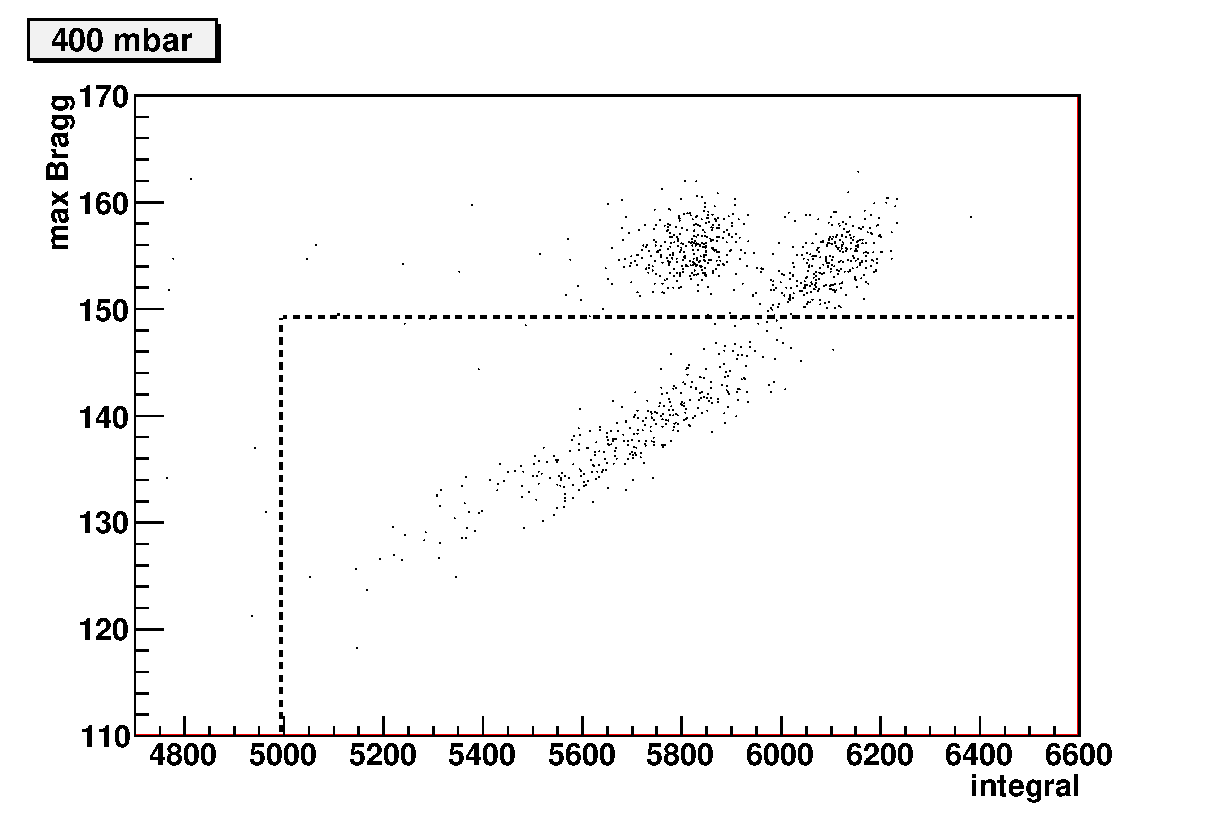
\includegraphics[width=0.8\textwidth]{400_max_integ.eps}
\caption{Grafico con valori degli integrali in ascissa e altezze dei picchi di Bragg in ordinata per gli eventi raccolti a \unit[400]{mbar}. La zona delimitata dalle righe tratteggiate racchiude gli eventi per cui le particelle $\a$ non sono state frenate nella camera.}
\label{max_integ}
\end{figure}
\newpage
Per questi eventi $\D t$ rappresenta il tempo impiegato dagli elettroni a percorrere la lunghezza della camera, per cui ne possiamo facilmente ricavare la velocit\`a di drift $v_e$, che assumeremo costante al variare della pressione.
\begin{align*}
v_e &= \frac{l}{\D t} = \unit[2.53 \pm 0.12]{cm/\micro s}\\
\beta_e &= \frac{v_e}{c} = 8.4 \cdot 10^{-5}
\end{align*}
dove $\D t = \unit[43.5 \pm 2]{canali}$ \`e la media dei tempi sugli eventi selezionati. Dato che la stima della durata dell'evento \`e influenzata dalla traiettoria della particella entro la camera, abbiamo considerato l'errore massimo di un canale sulla determinazione di ciascuno dei due istanti finale e iniziale, da cui l'incertezza di due canali su $\D t$. Da quest'ultima abbiamo calcolato l'errore su $v_e$, assumendo esatto il valore di $l$:
\begin{equation*}
\s(v_e) = \frac{v_e}{\D t} \s(\D t)
\end{equation*}

Infine vogliamo verificare che $v_e$ sia sempre molto minore della velocit\`a delle particelle $\a$. Quest'ultima diminuisce lungo il percorso, perci\`o scegliamo di farne una stima in corrispondenza del picco di Bragg.
% ma sappiamo che una volta raggiunto il picco di Bragg la particella ha praticamente perso il suo potere ionizzante. Di conseguenza possiamo assumere come valore minimo per $v_\a$ quello posseduto in corrispondenza del picco dalle emissioni del Pu alla pressione di \unit[600]{mbar}.
Osserviamo che, nel nostro caso, l'energia cinetica in tale istante \`e proporzionale all'integrale del segnale nell'intervallo $[0, t_{\max}]$. Possiamo allora calcolare la media $E_{\text{frac}}$ delle frazioni di energia residua per le emissioni del polonio a \unit[600]{mbar}, da cui
\begin{equation*}
\beta_\a = \frac{v_\a}{c} = \left[ \frac{2 E_{\text{frac}} E_\a}{m_a} \right]^{1/2} = 0.033
\end{equation*}
essendo $E_\a=\unit[5.148]{MeV}$ e $m_\a=\unit[3727.379]{MeV}$.\footnote{Fonte per $m_\a$: database \texttt{http://physics.nist.gov/cgi-bin/cuu/}}

Confrontando con $\beta_e$ calcolato sopra si verifica
\begin{equation*}
\beta_\a \gg \beta_e
\end{equation*}
\subsection{Range e verifica della legge di Bragg-Kleman}
Come per le grandezze analizzate precedentemente, abbiamo realizzato gli istogrammi con le occorrenze delle durate di ciascun evento, proporzionali al range delle particelle $\a$.
Riportiamo quello relativo alla pressione di \unit[550]{mbar}:
\begin{figure}[h!]\centering
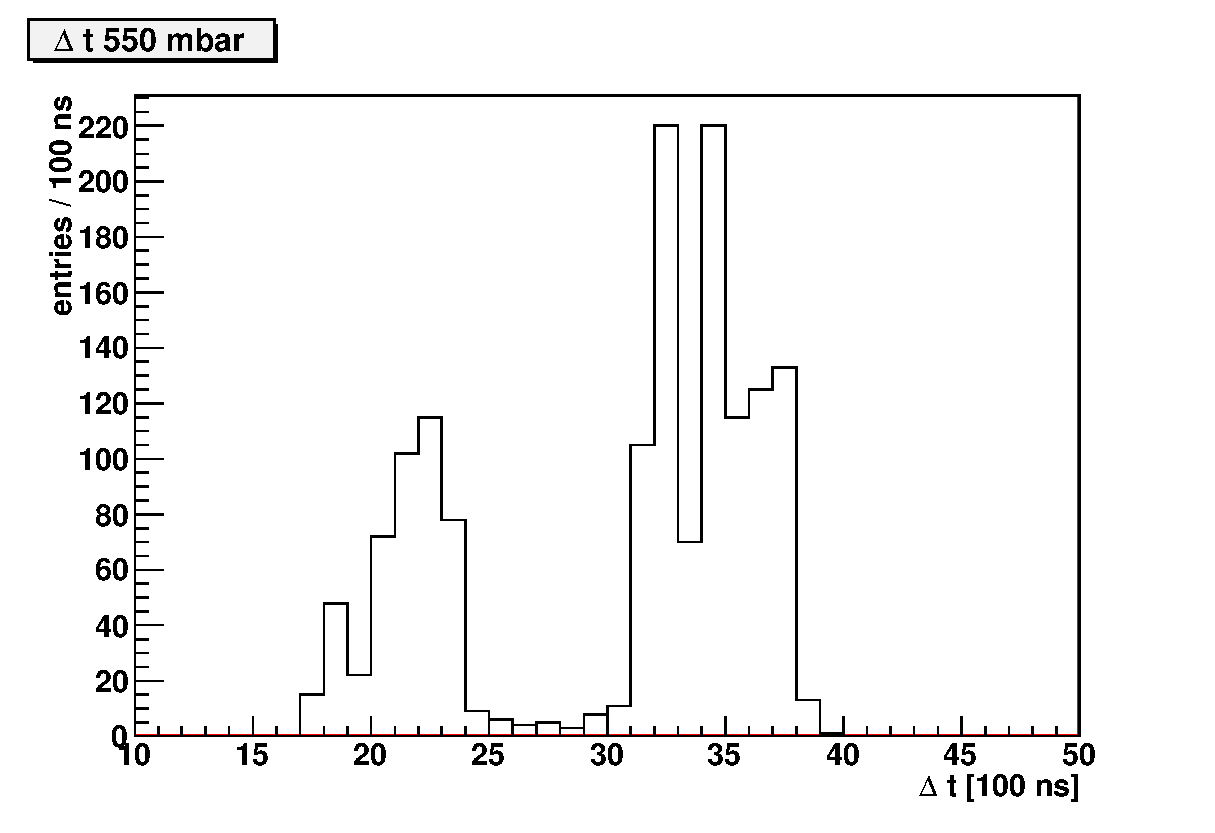
\includegraphics[width=0.8\textwidth]{550_range.eps}
\caption{Istogramma delle occorrenze dei valori $\D t$ di durata Abbiamo calcolato la media dei $\D t$ degli eventi dei singoli eventi, stimati come larghezza del segnale al 45~\% di altezza della curva. Si distinguono tre picchi distinti, relativi alle particelle emesse rispettivamente da Pu, Am, Cm. I dati si riferiscono alla pressione di \unit[550]{mbar}.}
\label{range_hist}
\end{figure}\\
Suddividendo gli eventi in base all'energia, abbiamo calcolato il valor medio, con relativo errore, di $\D t$ corrispondente a ciascuna emissione. Da questi, moltiplicando per la velocit\`a di drift degli elettroni $v_e = \unit[2.53]{cm/\micro s}$ calcolata al paragrafo precedente, si ottiene una stima del range $R$ delle particelle $\a$.

L'incertezza su $R$ \`e stimata come:
\begin{equation*}
\s(R) = \left[ v_e^2 \s^2(\D t) + \D t^2 \s^2(v_e) \right]^{1/2}
\end{equation*}
Riportiamo i risultati ottenuti in tabella~\ref{range}.
\begin{table}[h!]\centering
\renewcommand{\arraystretch}{1.2}
\begin{tabular}{cl*3{r@{ $\pm$ }l}}
$P$ (mbar)&		&	\multicolumn{2}{c}{\Pu}& \multicolumn{2}{c}{\Am}& \multicolumn{2}{c}{\Cm}\\\midrule[0.15em]
400&	$\D t$ (\unit[100]{ns})&	41.212 & 0.047&    	44.342 & 0.048&		\multicolumn{2}{c}{ } \\
&	$R$ (cm)&			10.41 & 0.48&    	11.20 & 0.51&	 	\multicolumn{2}{c}{ }\\\hline
450&	$\D t$&				37.497 &  0.047&	40.563 &  0.050&	43.323 &  0.045\\
&	$R$&				9.47 &  0.44&	10.24 &  0.47&	10.94 &  0.50\\\hline
500&	$\D t$&				34.168 &  0.043&	36.869 &  0.043&	39.588 &  0.042\\
&	$R$ &				8.63 &  0.40&	9.31 &  0.43&	10.00 &  0.46\\\hline
550&	$\D t$ &			31.720 &  0.036&	34.172 &  0.034&	36.594 &  0.043\\
&	$R$ &				8.01 &  0.37&	8.63 &  0.40&	9.24 &  0.42\\\hline
600&	$\D t$ &			29.916 &  0.035&	32.128 &  0.057&	34.141 &  0.052\\
&	$R$ &				7.56 &  0.35&	8.11 &  0.37&	8.62 &  0.40
\end{tabular}
\caption{Valori medi di $\D t$ e relative stime del range $R$ delle particelle $\a$.}
\label{range}
\end{table}\\
% La stima del range delle particelle per l'americio a \unit[400]{mbar} d\`a un valore superiore alla lunghezza della camera. Ci\`o pu\`o essere dovuto al fatto che parte di queste non vengono completamente frenate e 
\newpage
Nel nostro caso la legge di Bragg-Kleman si riduce a
\begin{equation*}
\frac{\D t_1}{\D t_2} = \frac{R_1}{R_2} = \frac{P_2}{P_1}
\end{equation*}
avendo studiato la propagazione in un gas di cui abbiamo fatto variare solo il parametro della pressione.

Per verificarne la validit\`a abbiamo calcolato le varie coppie di rapporti tra $P$ e $\D t$ e per ciascuna abbiamo stimato la compatibilit\`a tra i due valori. Gli errori sui rapporti $\D t_2 / \D t_1$ sono calcolati come:
\begin{equation*}
\s\left(\frac{\D t_2}{\D t_1}\right) = \left[ \left(\frac{\D t_2}{\D t_1^2}\: \s(\D t_1)\right)^2
+ \left(\frac{1}{\D t_1} \s(\D t_2)\right)^2\right]^{1/2}
\end{equation*}

\begin{table}[h!]\centering
\renewcommand{\arraystretch}{1.1}
\begin{tabular}{c@{ = }c|*2c|*2c|*2c}
\multicolumn{2}{c}{}	&	\multicolumn{2}{|c|}{\Pu}&	\multicolumn{2}{c|}{\Am}&	\multicolumn{2}{c}{\Cm}\\
\multicolumn{2}{c|}{$P_1 / P_2$}&	$\D t_2 / \D t_1$&	compat.&	$\D t_2 / \D t_1$&	compat.&	$\D t_2 / \D t_1$&	compat.\\\hline
600 / 550& 1.091&      	1.060 $\pm$ 0.037&     0.83&	1.064 $\pm$ 0.060&     	0.45&	1.072 $\pm$ 0.056&     0.34\\
600 / 500& 1.200&      	1.142 $\pm$ 0.040&     1.45&	1.148 $\pm$ 0.065&     	0.81&	1.160 $\pm$ 0.060&     0.67\\
600 / 450& 1.333&      	1.253 $\pm$ 0.044&     1.83&	1.263 $\pm$ 0.072&     	0.99&	1.269 $\pm$ 0.066&     0.98\\
600 / 400& 1.500&      	1.378 $\pm$ 0.048&     2.55&	1.380 $\pm$ 0.078&     1.53& 	& \\
550 / 500& 1.100&      	1.077 $\pm$ 0.039&     0.59&	1.079 $\pm$ 0.037&    	0.58&	1.082 $\pm$ 0.047&     0.39\\
550 / 450& 1.222&      	1.182 $\pm$ 0.043&     0.94&	1.187 $\pm$ 0.040&     	0.88&	1.184 $\pm$ 0.051&     0.75\\
550 / 400& 1.375&      	1.299 $\pm$ 0.047&     1.61&	1.298 $\pm$ 0.044&     1.76&	& \\
500 / 450& 1.111&      	1.097 $\pm$ 0.048&     0.29&	1.100 $\pm$ 0.047&     	0.23&	1.094 $\pm$ 0.046&     0.36\\
500 / 400& 1.250&      	1.206 $\pm$ 0.052&     0.84&	1.203 $\pm$ 0.052&     0.92&	& \\
450 / 400& 1.125&     	1.099 $\pm$ 0.051&     0.50&	1.093 $\pm$ 0.055&     0.58&	& \\
\end{tabular}
\caption{Compatibilit\`a tra i rapporti $P_1/P_2$ e $\D t_2/\D t_1$ per ciascuna coppia di pressioni.}
\end{table} 
Avendo ottenuto valori di compatibilit\`a ovunque buoni, possiamo ritenere verificata la legge di Bragg-Kleman.
\section{Algoritmi utilizzati}\label{macro}
Abbiamo cercato di migliorare leggermente le \emph{macro} di ROOT a
disposizione. Oltre alle modifiche ai limiti e alla larghezza dei canali
degli istogrammi descritte sopra, abbiamo cambiato il tipo della variabile
che rappresenta il fondo medio da \texttt{int} a \texttt{float} per evitare
errori sistematici dovuti all'arrotondamento.

Inoltre, al massimo di Bragg viene sottratto il fondo medio del relativo
istogramma e viene calcolata la frazione di energia residua dopo il massimo
di Bragg, utile per confrontare la velocità delle particelle alfa con quella
degli elettroni nel gas.

Le altre differenze sono solo frutto di una riscrittura e non modificano i
calcoli eseguiti. Tutto il codice, compreso il programma principale per
costruire gli alberi dai dati grezzi (\texttt{my\_bragg.cpp}) è disponibile all'indirizzo
\texttt{http://www.latinblog.org/programmi/macro.tar.gz}
\end{document}
